\chapter{PROJECT PLAN}

\section{Project Timeline}

Figure~\ref{fig:timeline} presents the 10-week project timeline for the \textit{Probabilistic Path Optimization using Pruned Dijkstra} project. Tasks are organized in three overlapping phases: implementation (Weeks~1--4), testing and experimentation (Weeks~4--7), and analysis, writing, and presentation (Weeks~7--10). This phased structure ensures that correctness is validated before experimentation begins, and that experimental results directly inform the final report and presentation.

\textbf{Current status:} The project is currently in the \textit{Experimental Execution and Analysis} stage (Weeks~5--7). Core implementation and unit testing have been completed; synthetic and real-data experiments have been executed and results are under analysis.

\begin{figure}[h!]
\centering
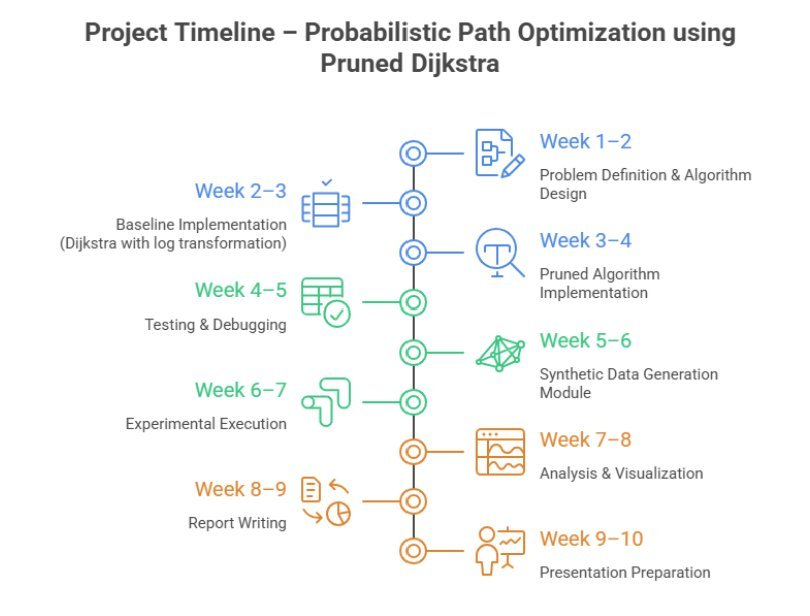
\includegraphics[width=0.85\textwidth]{timeline.png}
\caption[Project timeline]{Ten-week project timeline with implementation (blue), experimentation (green), and writing (orange) phases.}
\label{fig:timeline}
\end{figure}

Figure~\ref{fig:timeline} presents the 10-week project timeline, structured across three overlapping phases along a central spine. Blue entries (Weeks~1--4) cover core implementation, green entries (Weeks~4--7) cover testing and experimentation, and orange entries (Weeks~7--10) correspond to writing and presentation. Each phase overlaps with the next to allow iterative refinement of results and documentation.

\section{Milestones}

The project is structured around four key milestones. The first milestone, \textbf{Core Implementation}, was completed by the end of Week~4: both the baseline Dijkstra algorithm and the probability-pruned Dijkstra variant were fully implemented, tested on small hand-computed graphs, and validated for correctness against ground-truth optimal paths. The second milestone, \textbf{Experiments}, is targeted for completion by the end of Week~7; all experimental runs across small, medium, and large graph configurations are being executed, with all metrics (execution time, peak memory, nodes explored, edges relaxed, optimality gap, MaxPQSize) recorded and verified. The third milestone, \textbf{Report Completion}, is scheduled for the end of Week~9, at which point the full project report will be finalised incorporating experimental results, visualisations, complexity validation, and the time--memory--optimality trade-off discussion. The fourth milestone, \textbf{Final Presentation}, targets Week~10, when presentation slides and a live demonstration of the implementation will be prepared for the final project presentation on 12~March~2026.
